\documentclass[a4paper,12pt]{article}
   % Packages and definitions:
   % {
      \usepackage{float}
      \usepackage[english]{babel}
      \usepackage[utf8]{inputenc}
      \usepackage{amsmath}
      \usepackage{amssymb}
      \usepackage{color}
      \usepackage{subcaption}
      \usepackage{booktabs}
      \usepackage{tikz}
      \usepackage{multirow}
      \usetikzlibrary{decorations.pathreplacing}
      \usepackage{graphicx,epstopdf}
      \usepackage{cleveref}
      \usepackage{collcell} % loads array
      \usepackage{listings}
      \usepackage{algorithm}
      \usepackage{algpseudocode}
      \newcolumntype{m}{>{$} r <{$}}
      \newcolumntype{u}{>{$[\collectcell\si} l <{\endcollectcell]$}}
      \newcommand{\approxtext}[1]{\ensuremath{\stackrel{\text{#1}}{=}}}
      \newcommand{\matr}[1]{\mathbf{#1}}
      \newcommand{\partt}[2]{\ensuremath{\dfrac{\d {#1}}{\partial {#2}}}}
      \renewcommand{\d}[1]{\ensuremath{\operatorname{d}\!{#1}}} % non-italized differentials
      \newcommand{\h}[0]{\ensuremath{\hbar}} % hbar
      \newcommand{\qed}[0]{\ensuremath{\tag*{$\square$}}} % QED square
      \def\changemargin#1#2{\list{}{\rightmargin#2\leftmargin#1}\item[]}
      \let\endchangemargin=\endlist 
      \usepackage{amsthm}
      \theoremstyle{plain}
      \newtheorem{thm}{theorem} % reset theorem numbering for each chapter
      \theoremstyle{definition}
      \newtheorem{defn}[thm]{definition} % definition numbers are dependent on theorem numbers
      \newtheorem{exmp}[thm]{example} % same for example numbers
      \bibliographystyle{natbib}
      \renewcommand{\theequation}{\thesection.\arabic{equation}}
      \newcommand{\ts}{\textsuperscript} 

      \definecolor{dkgreen}{rgb}{0,0.6,0}
      \definecolor{gray}{rgb}{0.5,0.5,0.5}
      \definecolor{mauve}{rgb}{0.58,0,0.82}

      \lstset{frame=tb,
        language=Java,
        aboveskip=3mm,
        belowskip=3mm,
        showstringspaces=false,
        columns=flexible,
        basicstyle={\small\ttfamily},
        numbers=none,
        numberstyle=\tiny\color{gray},
        keywordstyle=\color{blue},
        commentstyle=\color{dkgreen},
        stringstyle=\color{mauve},
        breaklines=true,
        breakatwhitespace=true,
        tabsize=3
      }
% }
\title
{
	\textbf
	{
   On the warring of ants: Modelling competitive ant colonization through random walks
   }
}

\author{Henrik Åhl\\
\small{in collaboration with Denhanh Huynh}}
\date{\today}

\begin{document}
\begin{titlepage}
	
   \maketitle 
	\begin{center}
		\phantom{a}
		{Department of Astronomy and Theoretical Physics, Lund University}
		\\[2cm]
		{Project supervised by Tobias Ambjörnsson}
		\vfill
		\includegraphics[height=4cm]{logocLUeng.pdf}
	\end{center}
	\thispagestyle{empty} % do not count pages just yet
\end{titlepage}
\section{Introduction}
   How animals and insects move is seldom truly something stochastic, although
   random walks can in some cases be used to mimic an overall behaviour that can
   be meaningful for larger populations, where the inherent structure is lost
   in noise.~\cite{midges} Indeed, also the use of stochastical methods on ant
   colonies have been done before, with respect to the complex underlying
   network therein~\cite{ants}. In this report we instead investigate the dynamics of a
   system where the competitve nature between different ant breeds play into
   account; two types of ants entitled \texttt{speedAnts} and \texttt{bruteAnts}
   are set out within a grid-based forest to gather food, build up new anthills and 
   make sure to survive battles with ants of different types. The both types
   within our model are characterized by different values in the the two attributes 
   \emph{speed} and \emph{strength} corresponding to their respective names.  

   Several collective stochastical processes play deeply into the dynamics of the
   system. In particular, the walks of the ants are determined by a random direction,
   biased in the direction of food sources if the ant is not already carrying
   food, or strongly biased towards friendly anthills if not. 

\newpage

\section{Creating a model for colonization}
	\setcounter{equation}{0}
   \subsection{Problem description}
      We do in this report try to determine several things with respect to the
      dynamics of our model. Mainly we want to investigate how the attributes
      play into the evolution of the system with time. Secondly, as a direct
      consequence, it is of interest too see whether there can be established
      local equilibriums, where both ants stagnate in development. Due to the
      high chaotic nature of the model it is unlikely that a final equilibrium
      will be reached, why the occurence of local ones is of greater interest.   
      Also the forest size should affect which ant type is or is not at a loss,
      and how the system develops.
   
   \subsection{Description of the model}
      In essence, the model created to simulate the dynamics is centered around
      five steps, summarized as follows:
      \begin{enumerate}
         \item Add new food to grid.
         \item Let ants of different types combat when standing on the same
            square.
         \item Move ants to an adjacent square, or stay within the initial one.
         \item Let ants who stand on squares with food collect.
         \item Update anthills and leave off food. If food supply is big enough, 
            create a new anthill. Also generate new ants.
      \end{enumerate}
      As a practice for our simulations, the number of anthills that could be
      present within the forest was set at a maximum level to avoid diverging
      dynamics. 

   \subsection{Where to go: How ants walk}
      Ant walk biases are determined by the speed inherent to their type, as well
      as a summation over their different biases -- food supplies for ants not 
      carrying food, and friendly anthills for ants with food. These biases are
      weighed with respect to the inverse of their distance to the ant squared,
      so that the ant more securely walks in the correct direction the closer it
      gets to its target. All ants do, however, have a chance not to move during
      the time step, but rather spend time within its present square. This too
      is scaled in relation to the speed of the ant type, so that a quicker type
      will be less likely to stand still during its turn as an effect. The
      details of this procedure can be found in \cref{sec:code} under the method
      \texttt{move}.

   \subsection{Brawling in nature: How ants fight}
      Whenever two or more ants of opposing sides happen to stand upon the same
      square, combat will commence. The result of combat is drawn from two
      non-negative Gaussian distributions, where each distribution corresponds
      to how many ants of the opposing side the ants manage to kill. In essence,
      whenever a value $<0$ is drawn, it is substituted for a new one. The mean
      is centered around the sum of the total strength of an ant type, whereas
      the standard deviation is the root of this, making it likely that
      the number of ants killed by a species is roughly the same as their
      cumulative strength. For further reference, code is included in
      \cref{sec:code} under the method \texttt{combat}.
   
   \subsection{Simulation settings}
      Food is distributed randomly across the grid with a 1~\% chance. In total
      up to three stacks of food will be placed per occurence of this sort, although
      it is still possible for more food to appear before the other supplies
      have vanquished. The amount of food is drawn from a uniform distribution,
      where the range stretches between 0--15000 units. 

      All anthills generate one new ant per time step. Whenever the supply of
      nutrition in a separate hill has reached over 8000 units, the hill will 
      migrate to a nearby neighborhood, where the specific position is determined by a
      uniform distribution. Furthermore, a ceiling was set at 25 anthills in
      total throughout the forest in order to limit the system numerically.

\section{Results and conclusions}
      It is clear from the results that the matrix size, i.e. how big the
      modelized forest happens to be, is detrimental to the results of the
      dynamics throughout a simulation. It is clear that \texttt{bruteAnts} are
      favored by smaller matrices, where interactions are more regular and the
      competitiveness for the food sources is stronger. \texttt{speedAnts} are
      in turn favored by the larger maps, where interactions are sparse and
      development is largely determined by your ability to collect food.

      As can be seen in \cref{fig:lower} and \cref{fig:higher}, the system is
      largely determined by the size of the matrix. A larger grid allows for a
      smoother development, even though it is expected of the system to converge
      against a one-type scenario, where only one ant type de facto survives.
      Somewhere around the range of a $25\times 25$ matrix there seems to be a
      turning point where \texttt{speedAnts} are more favored by the
      environment, and \texttt{bruteAnts} fall behind.

      Notably, with respect to combat, in the sudden decrease in ants for both types in
      \cref{fig:higher}, \texttt{speedAnts} make up for their lack in strength through
      greater numbers, making larger combats fairly equal. The reader should
      take note howsoever, that this fact is purely inherent to the settings
      chosen when simulating, although it still shows the effect of allowing for
      numbers and flexibility to counter pure force in a dynamic system such as
      this.
   
      \begin{figure}[H]
         \vspace*{1cm}
         \hspace*{-2cm}
         \centering
         \begin{minipage}[t]{.6\textwidth}		
            \vspace{0pt}
            \centering
            \resizebox{\columnwidth}{!}{% GNUPLOT: LaTeX picture with Postscript
\begingroup
  \makeatletter
  \providecommand\color[2][]{%
    \GenericError{(gnuplot) \space\space\space\@spaces}{%
      Package color not loaded in conjunction with
      terminal option `colourtext'%
    }{See the gnuplot documentation for explanation.%
    }{Either use 'blacktext' in gnuplot or load the package
      color.sty in LaTeX.}%
    \renewcommand\color[2][]{}%
  }%
  \providecommand\includegraphics[2][]{%
    \GenericError{(gnuplot) \space\space\space\@spaces}{%
      Package graphicx or graphics not loaded%
    }{See the gnuplot documentation for explanation.%
    }{The gnuplot epslatex terminal needs graphicx.sty or graphics.sty.}%
    \renewcommand\includegraphics[2][]{}%
  }%
  \providecommand\rotatebox[2]{#2}%
  \@ifundefined{ifGPcolor}{%
    \newif\ifGPcolor
    \GPcolorfalse
  }{}%
  \@ifundefined{ifGPblacktext}{%
    \newif\ifGPblacktext
    \GPblacktexttrue
  }{}%
  % define a \g@addto@macro without @ in the name:
  \let\gplgaddtomacro\g@addto@macro
  % define empty templates for all commands taking text:
  \gdef\gplbacktext{}%
  \gdef\gplfronttext{}%
  \makeatother
  \ifGPblacktext
    % no textcolor at all
    \def\colorrgb#1{}%
    \def\colorgray#1{}%
  \else
    % gray or color?
    \ifGPcolor
      \def\colorrgb#1{\color[rgb]{#1}}%
      \def\colorgray#1{\color[gray]{#1}}%
      \expandafter\def\csname LTw\endcsname{\color{white}}%
      \expandafter\def\csname LTb\endcsname{\color{black}}%
      \expandafter\def\csname LTa\endcsname{\color{black}}%
      \expandafter\def\csname LT0\endcsname{\color[rgb]{1,0,0}}%
      \expandafter\def\csname LT1\endcsname{\color[rgb]{0,1,0}}%
      \expandafter\def\csname LT2\endcsname{\color[rgb]{0,0,1}}%
      \expandafter\def\csname LT3\endcsname{\color[rgb]{1,0,1}}%
      \expandafter\def\csname LT4\endcsname{\color[rgb]{0,1,1}}%
      \expandafter\def\csname LT5\endcsname{\color[rgb]{1,1,0}}%
      \expandafter\def\csname LT6\endcsname{\color[rgb]{0,0,0}}%
      \expandafter\def\csname LT7\endcsname{\color[rgb]{1,0.3,0}}%
      \expandafter\def\csname LT8\endcsname{\color[rgb]{0.5,0.5,0.5}}%
    \else
      % gray
      \def\colorrgb#1{\color{black}}%
      \def\colorgray#1{\color[gray]{#1}}%
      \expandafter\def\csname LTw\endcsname{\color{white}}%
      \expandafter\def\csname LTb\endcsname{\color{black}}%
      \expandafter\def\csname LTa\endcsname{\color{black}}%
      \expandafter\def\csname LT0\endcsname{\color{black}}%
      \expandafter\def\csname LT1\endcsname{\color{black}}%
      \expandafter\def\csname LT2\endcsname{\color{black}}%
      \expandafter\def\csname LT3\endcsname{\color{black}}%
      \expandafter\def\csname LT4\endcsname{\color{black}}%
      \expandafter\def\csname LT5\endcsname{\color{black}}%
      \expandafter\def\csname LT6\endcsname{\color{black}}%
      \expandafter\def\csname LT7\endcsname{\color{black}}%
      \expandafter\def\csname LT8\endcsname{\color{black}}%
    \fi
  \fi
  \setlength{\unitlength}{0.0500bp}%
  \begin{picture}(7200.00,5040.00)%
    \gplgaddtomacro\gplbacktext{%
      \colorrgb{0.42,0.42,0.42}%
      \put(1210,704){\makebox(0,0)[r]{\strut{} 0}}%
      \colorrgb{0.42,0.42,0.42}%
      \put(1210,1518){\makebox(0,0)[r]{\strut{} 5000}}%
      \colorrgb{0.42,0.42,0.42}%
      \put(1210,2332){\makebox(0,0)[r]{\strut{} 10000}}%
      \colorrgb{0.42,0.42,0.42}%
      \put(1210,3147){\makebox(0,0)[r]{\strut{} 15000}}%
      \colorrgb{0.42,0.42,0.42}%
      \put(1210,3961){\makebox(0,0)[r]{\strut{} 20000}}%
      \colorrgb{0.42,0.42,0.42}%
      \put(1210,4775){\makebox(0,0)[r]{\strut{} 25000}}%
      \colorrgb{0.42,0.42,0.42}%
      \put(1342,484){\makebox(0,0){\strut{} 0}}%
      \colorrgb{0.42,0.42,0.42}%
      \put(2252,484){\makebox(0,0){\strut{} 500}}%
      \colorrgb{0.42,0.42,0.42}%
      \put(3162,484){\makebox(0,0){\strut{} 1000}}%
      \colorrgb{0.42,0.42,0.42}%
      \put(4073,484){\makebox(0,0){\strut{} 1500}}%
      \colorrgb{0.42,0.42,0.42}%
      \put(4983,484){\makebox(0,0){\strut{} 2000}}%
      \colorrgb{0.42,0.42,0.42}%
      \put(5893,484){\makebox(0,0){\strut{} 2500}}%
      \colorrgb{0.42,0.42,0.42}%
      \put(6803,484){\makebox(0,0){\strut{} 3000}}%
      \colorrgb{0.42,0.42,0.42}%
      \put(176,2739){\rotatebox{-270}{\makebox(0,0){\strut{}Living ants}}}%
      \colorrgb{0.42,0.42,0.42}%
      \put(4072,154){\makebox(0,0){\strut{}Time}}%
      \colorrgb{0.42,0.42,0.42}%
      \put(4072,4665){\makebox(0,0){\strut{}}}%
    }%
    \gplgaddtomacro\gplfronttext{%
      \csname LTb\endcsname%
      \put(5804,4602){\makebox(0,0)[r]{\strut{}speedAnts, 25}}%
      \csname LTb\endcsname%
      \put(5804,4382){\makebox(0,0)[r]{\strut{}bruteAnts, 25}}%
      \csname LTb\endcsname%
      \put(5804,4162){\makebox(0,0)[r]{\strut{}speedAnts, 5}}%
      \csname LTb\endcsname%
      \put(5804,3942){\makebox(0,0)[r]{\strut{}bruteAnts, 5}}%
    }%
    \gplbacktext
    \put(0,0){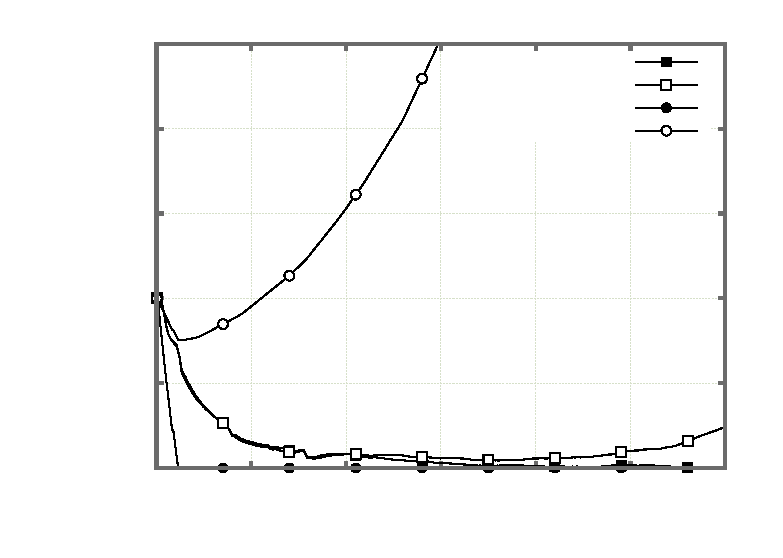
\includegraphics{lower}}%
    \gplfronttext
  \end{picture}%
\endgroup
}
            \caption{Comparison of dynamics between matrix with side 5 and side
            25.}
             \label{fig:lower}
         \end{minipage}~\hspace*{1em}
         \begin{minipage}[t]{.6\textwidth}		
            \vspace{0pt}
            \centering
            \resizebox{\columnwidth}{!}{% GNUPLOT: LaTeX picture with Postscript
\begingroup
  \makeatletter
  \providecommand\color[2][]{%
    \GenericError{(gnuplot) \space\space\space\@spaces}{%
      Package color not loaded in conjunction with
      terminal option `colourtext'%
    }{See the gnuplot documentation for explanation.%
    }{Either use 'blacktext' in gnuplot or load the package
      color.sty in LaTeX.}%
    \renewcommand\color[2][]{}%
  }%
  \providecommand\includegraphics[2][]{%
    \GenericError{(gnuplot) \space\space\space\@spaces}{%
      Package graphicx or graphics not loaded%
    }{See the gnuplot documentation for explanation.%
    }{The gnuplot epslatex terminal needs graphicx.sty or graphics.sty.}%
    \renewcommand\includegraphics[2][]{}%
  }%
  \providecommand\rotatebox[2]{#2}%
  \@ifundefined{ifGPcolor}{%
    \newif\ifGPcolor
    \GPcolorfalse
  }{}%
  \@ifundefined{ifGPblacktext}{%
    \newif\ifGPblacktext
    \GPblacktexttrue
  }{}%
  % define a \g@addto@macro without @ in the name:
  \let\gplgaddtomacro\g@addto@macro
  % define empty templates for all commands taking text:
  \gdef\gplbacktext{}%
  \gdef\gplfronttext{}%
  \makeatother
  \ifGPblacktext
    % no textcolor at all
    \def\colorrgb#1{}%
    \def\colorgray#1{}%
  \else
    % gray or color?
    \ifGPcolor
      \def\colorrgb#1{\color[rgb]{#1}}%
      \def\colorgray#1{\color[gray]{#1}}%
      \expandafter\def\csname LTw\endcsname{\color{white}}%
      \expandafter\def\csname LTb\endcsname{\color{black}}%
      \expandafter\def\csname LTa\endcsname{\color{black}}%
      \expandafter\def\csname LT0\endcsname{\color[rgb]{1,0,0}}%
      \expandafter\def\csname LT1\endcsname{\color[rgb]{0,1,0}}%
      \expandafter\def\csname LT2\endcsname{\color[rgb]{0,0,1}}%
      \expandafter\def\csname LT3\endcsname{\color[rgb]{1,0,1}}%
      \expandafter\def\csname LT4\endcsname{\color[rgb]{0,1,1}}%
      \expandafter\def\csname LT5\endcsname{\color[rgb]{1,1,0}}%
      \expandafter\def\csname LT6\endcsname{\color[rgb]{0,0,0}}%
      \expandafter\def\csname LT7\endcsname{\color[rgb]{1,0.3,0}}%
      \expandafter\def\csname LT8\endcsname{\color[rgb]{0.5,0.5,0.5}}%
    \else
      % gray
      \def\colorrgb#1{\color{black}}%
      \def\colorgray#1{\color[gray]{#1}}%
      \expandafter\def\csname LTw\endcsname{\color{white}}%
      \expandafter\def\csname LTb\endcsname{\color{black}}%
      \expandafter\def\csname LTa\endcsname{\color{black}}%
      \expandafter\def\csname LT0\endcsname{\color{black}}%
      \expandafter\def\csname LT1\endcsname{\color{black}}%
      \expandafter\def\csname LT2\endcsname{\color{black}}%
      \expandafter\def\csname LT3\endcsname{\color{black}}%
      \expandafter\def\csname LT4\endcsname{\color{black}}%
      \expandafter\def\csname LT5\endcsname{\color{black}}%
      \expandafter\def\csname LT6\endcsname{\color{black}}%
      \expandafter\def\csname LT7\endcsname{\color{black}}%
      \expandafter\def\csname LT8\endcsname{\color{black}}%
    \fi
  \fi
  \setlength{\unitlength}{0.0500bp}%
  \begin{picture}(7200.00,5040.00)%
    \gplgaddtomacro\gplbacktext{%
      \colorrgb{0.42,0.42,0.42}%
      \put(1210,704){\makebox(0,0)[r]{\strut{} 0}}%
      \colorrgb{0.42,0.42,0.42}%
      \put(1210,1518){\makebox(0,0)[r]{\strut{} 5000}}%
      \colorrgb{0.42,0.42,0.42}%
      \put(1210,2332){\makebox(0,0)[r]{\strut{} 10000}}%
      \colorrgb{0.42,0.42,0.42}%
      \put(1210,3147){\makebox(0,0)[r]{\strut{} 15000}}%
      \colorrgb{0.42,0.42,0.42}%
      \put(1210,3961){\makebox(0,0)[r]{\strut{} 20000}}%
      \colorrgb{0.42,0.42,0.42}%
      \put(1210,4775){\makebox(0,0)[r]{\strut{} 25000}}%
      \colorrgb{0.42,0.42,0.42}%
      \put(1342,484){\makebox(0,0){\strut{} 0}}%
      \colorrgb{0.42,0.42,0.42}%
      \put(2252,484){\makebox(0,0){\strut{} 500}}%
      \colorrgb{0.42,0.42,0.42}%
      \put(3162,484){\makebox(0,0){\strut{} 1000}}%
      \colorrgb{0.42,0.42,0.42}%
      \put(4073,484){\makebox(0,0){\strut{} 1500}}%
      \colorrgb{0.42,0.42,0.42}%
      \put(4983,484){\makebox(0,0){\strut{} 2000}}%
      \colorrgb{0.42,0.42,0.42}%
      \put(5893,484){\makebox(0,0){\strut{} 2500}}%
      \colorrgb{0.42,0.42,0.42}%
      \put(6803,484){\makebox(0,0){\strut{} 3000}}%
      \colorrgb{0.42,0.42,0.42}%
      \put(176,2739){\rotatebox{-270}{\makebox(0,0){\strut{}Living ants}}}%
      \colorrgb{0.42,0.42,0.42}%
      \put(4072,154){\makebox(0,0){\strut{}Time}}%
      \colorrgb{0.42,0.42,0.42}%
      \put(4072,4665){\makebox(0,0){\strut{}}}%
    }%
    \gplgaddtomacro\gplfronttext{%
      \csname LTb\endcsname%
      \put(5804,4602){\makebox(0,0)[r]{\strut{}speedAnts, 100}}%
      \csname LTb\endcsname%
      \put(5804,4382){\makebox(0,0)[r]{\strut{}bruteAnts, 100}}%
      \csname LTb\endcsname%
      \put(5804,4162){\makebox(0,0)[r]{\strut{}speedAnts, 50}}%
      \csname LTb\endcsname%
      \put(5804,3942){\makebox(0,0)[r]{\strut{}bruteAnts, 50}}%
    }%
    \gplbacktext
    \put(0,0){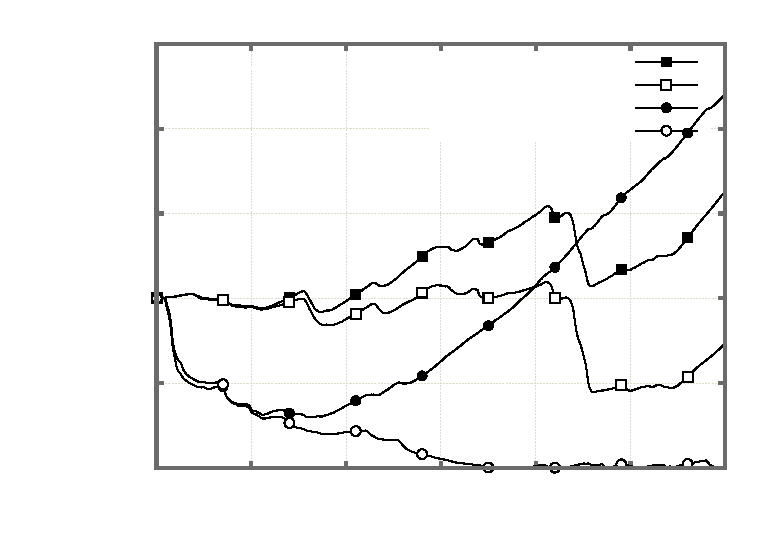
\includegraphics{higher}}%
    \gplfronttext
  \end{picture}%
\endgroup
}
            \caption{Comparison between matrix with side 50 and side 100}
            \label{fig:higher}
         \end{minipage}
      \end{figure}
      
      In order to verify the accuracy of the model, the graphical representation
      illustrated in \cref{fig:graph} below figured as an important measure. Accordingly 
      to the graphical output, no typical anomalies could be seen, which enhances the 
      belief that the model indeed did behave as intended.

      \begin{figure}[H]
         \centering
         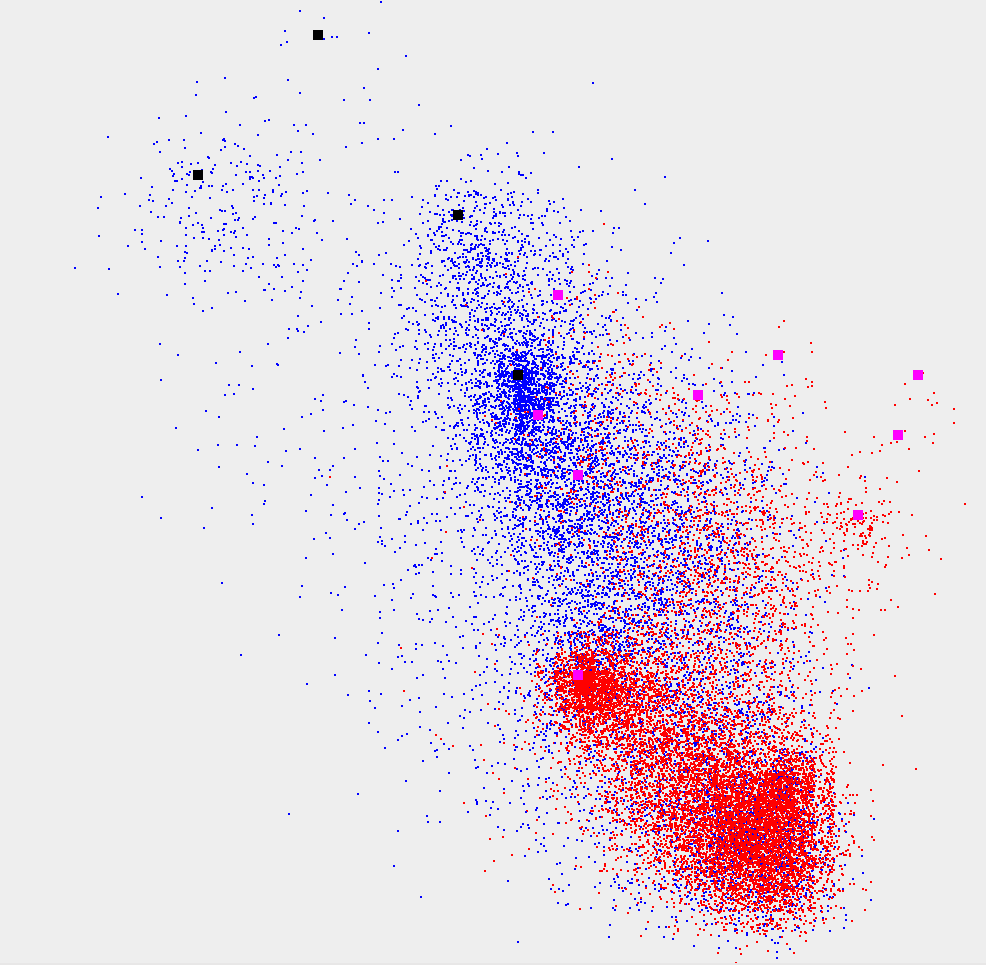
\includegraphics[width=.8\textwidth]{5050foodhunt.png}
         \caption{Snapshot of simulation in a $50 \times 50$ matrix.
            \texttt{speedAnts} are represented with blue dots (black anthills), while
            \texttt{bruteAnts} are seen as red (magenta anthills). In this capture, ants are seen
            having just finished a source of food, and are returning homeward.} 
         \label{fig:graph}            
      \end{figure}

      Contrary to the initial aim of investigation, there seems to be some
      possibilities of establishing local equilibriums, where both types of ants
      can live on for an extended amount of time. Especially the $50 \times 50$ matrix
      simulation visualized in \cref{fig:higher} displays this behaviour.

      However, also the amount of ants with which the system is first initialized
      with, as well as the amount of food spawned (and in how many places)
      can gravely shift the stability of how the system develops. 

      In summary, the dynamics of such a highly stochastic system are hard to
      properly measure and compare. The severe fluctuations that are inherent to
      the model, and the demanding computations that forelie makes statistical
      checks within the thermodynamical limit practically impossible. The
      system may act as a model for how stochastical principles can determine
      the nature of such a system as this, although it can not be deemed to be
      of any practical importance. 

\newpage

\begin{thebibliography}{99}
   \bibitem{lecnotes}
     Tobias Ambjörnsson,
     \emph{Lecture notes, Computational Physics},
     Department of Astronomy and Theoretical Physics,
     Lund University,
     2015.
  \bibitem{midges}
      A. Attanasi et al,
      \emph{Collective Behaviour without Collective Order in Wild Swarms of
      Midges},
      PLoS Computational Biology: 10(7),
      2014.
   \bibitem{ants}
      D. Jin et al,
      \emph{Ant Colony Optimization with a new Random Walk Model for Community
      Detection in Complex Networks},
      Jilin University,
      2013.
\end{thebibliography}
\newpage
\appendix
\section{Code}
   \label{sec:code}
   \lstinputlisting[language=Java]{Common.java}
   \lstinputlisting[language=Java]{Forest.java}
   \lstinputlisting[language=Java]{Square.java}
   \lstinputlisting[language=Java]{Food.java}
   \lstinputlisting[language=Java]{Anthill.java}
   \lstinputlisting[language=Java]{AntPanel.java}
   \lstinputlisting[language=Java]{Ant.java}
   \lstinputlisting[language=Java]{SpeedAnt.java}
   \lstinputlisting[language=Java]{BruteAnt.java}
\end{document}

